\chapter{Solution}
\label{ch:Model}

% We [outline|describe|introduce] our [proposed] [solution|model], [justify] design decisions and [implementation details| detail implementation| document implementation details].
In this chapter, we describe our solution, justify design decisions and detail implementation.


% An scheme of the solution is found there and we do it here...

\section{Task definition}
We segment digital mammograms into two separate regions: breast mass (benign or malignant) and general tissue.
Breast area is previously separated from the background by simple thresholding.
In particular, we train a convolutional network to estimate the probability of each pixel belonging to a mass and use these values to generate a valid segmentation.
%The breast area is separated from the background by simple thresholding.
%Background and breast area are separated using thresholded to zero.

% Maybe order as in
% Experiment 1 (architecture 1)
%		Hyperparamtere search
% Experiment 2 (architecture 1, weighted loss)
%		Hyperparameter search
% Experiment 3 (architecture 2, maybe weighted loss)
%		Hyperparameter search

\section{Data set}
%We document the retrieval, enhancement, labelling and augmentation of [the|our] data set [used for the experiments].
% We document how we retrieve, enhance, label and augment our data set.
We document the retrieval, enhancement, labelling and augmentation of our data set.

\subsection{Database}
We use the Breast Cancer Digital Repository (BCDR-DM) database. In particular, we use the BDCR-D01 data set, which is composed of patients with at least one breast mass. We have curated it to delete patients with breast implants or other extraneous features ().

We select x digital mammograms from x patients. Theya are 8-bit images with 0.07mm spatial resolution whose size is ta, ta or ta, depending on the size of the placa used to obtain the pictures. Each lesion is segmented and its ... (labels), ..., ..., ... is supplied. Other patient data and image features are supplied but we do not make use of them.
% Files and how are they organized. Data available per case and per mammogram. How are boundaries written. formats, etc.

Digital mammograms have higher image quality and lack any marks, stamps or other scanning artifacts present in digitized film mammograms; this allows us to pick up better features and eases segmentation. Although the number of mammograms is small, training on overlapping patches and data augmentation, allows learning.


\subsection{Data division}
70/15/15 is a good split. stratified per patient, this total number of patients in each set and this total number of mammograms (after augmentation) and this total number of lesions.

\begin{table}[h]
	\centering
	\begin{tabular}{ccccc}
		\hline
		&\textbf{Training} & \textbf{Validation} & \textbf{Test} & \textbf{Total}\\
		\hline 
		\textbf{Percentage of data set}	&70	&15	&15	&100\\
		\textbf{Number of patients} &43&10&10&63\\
		\textbf{Number of mammograms} &180&38&38&256\\
		\textbf{Number of masses} &97&21&21&139\\
		\textbf{Mammograms (after augmentation)} &1440&304&38&1782\\
		\hline
	\end{tabular}
	\caption[Data set summary]{Data set summary}
\end{table}

\subsection{Image dimensions}
We decided to hold xbyx cm to hold an entire mass.

% Masses are 12.2mm + 4.5mm std . 2 cm holds 96% of masses. 1.5 holds 73 % of masses
That's hwta they say and also by visual inspection ins ome triaing examples


We use square image patches because they are common in practice and simplify data augmentation. To define the size we have to consider two aspects: keeping a manageable input size for the network (in pixels) and capturing the entire lesion in the image patch (in mm).

The smallest microcalcification worth considering could be as small as 0.16 mm~\cite{Lo1998}, thus the spatial resolution should be at most 0.16 mm. The standard definition of a cluster of microcalcifications is of 5 or more inside a 1 $cm^2$ area~\cite{Sickles2013}, thus the entire image patch should cover at least a 1 $cm^2$ area. Using an image patch of $64  \times 64$ pixels we cover an image area of 1 $cm^2$ with a pixel size of 0.156 mm. 
% Pizel size .16 , i get 1.024 cm size.
Mass sizes (length of the long axis) vary from 5 mm to 20 mm~\cite{Sahiner1996}~\footnote{Bigger masses are easily detectable by touch and thus less important for our purposes.} There is not really any restriction on spatial resolution other than it being good enough to capture texture information. Again, using an image size of $64 \times 64$ pixels we can cover a 4 $cm^2$ area (2 cm per side) with a spatial resolution of 0.313 mm.
% pixel size 0.39 equals area 25 mm
% pixel size .4 mm equals ara 25.6 mm (exactly the size in Sahiner1996)

The low spatial resolution (big pixel sizes), however, reduces the quality of the input images. An alternative could be to use $127 \times 127$ image patches with 0.079 mm and 0.157 mm pixel sizes for microcalcifications and masses, respectively, aplying a bigger filter on the first convolutional layer, for instance, a $5 \times 5$ filter with stride 2 and padding 2. This allows us to have bigger input images with a negligible increase in the number of parameters. Whether the results improve or not is not clear at this point.

Although we use the same input size (either $64 \times 64$ or $127 \times 127$) for microcalcifications and masses they do not cover the same area in the mammogram. We need to use two different sizes because if we preserve the spatial resolution of microcalcifications, the 1 $cm^2$ area would not be able to contain the entire mass meanwhile if we use a resolution closer to the one used for masses, small microcalcifications will dissapear and the 4 $cm^2$ area would have way too much noise compared to the size of the cluster of microcalcifications.
%An alternative is to use a $128 \times 128$ pixels image patch with 0.16 mm, this will result on the same 4 $cm^2$ area needed for masses with the spatial resolution needed for microcalcifications allowing us to train a single network for both kinds of lesions. Nonetheless, this has some critical flaws: the number of learnable parameters will almost double, the GPU may run into memory bottlenecks because of the increased number of parameters and unnnecesary details (noise) will be included in the image.

This dictates the spatial dimensions on our input volume in our convolutional network. The amount of pooling in the architecture defines the stride (and thus the amount of overlapping) during training.

We chose a stride of 3 mm. This is midway between a very small stride, say 0.05 mm, which produces many image patches with maximum overlapping and a big stride, say 1 cm, which produces fewer patches with little to no overlapping. We use a rather small stride to have a lesion appear in various image patches (although in a slightly different place in each one) and to produce a good number of patches from the original image (around 1K per mammogram). We use no padding.

When sliding the window starting from the upper left corner of the original image it is possible that due to a dimension mismatch pixels in the rightmost and bottom strips do not appear in any image patch, this is not a problem given that the lost strips are very thin ($<$ 3 mm) and they are normally part of the black background.

\paragraph{Resizing}
We have to resize the images to achieve the desired patch size. There is a couple of decisions to take in this part: the type of interpolation to use and whether image enhancement should be performed before or after resizing. After some experiments neither decisions proved to be very important for the resulting image patches. We choose the Lanczos interpolation recommended for downsizing in the PILLOW Python Image Library. Enhancements are executed on each particular patch before being scaled to their final size. Figure~\ref{fig:ResizingInterps} shows the effect of using the Bicubic or Lanczos interpolation scheme for resizing both before and after enhancement. Results are similar under all configurations.
% Make sure you store them when resized as a single channel grayscale image, maybe png. Otherwise it will be stored as color image.

\begin{figure}
	\centering
	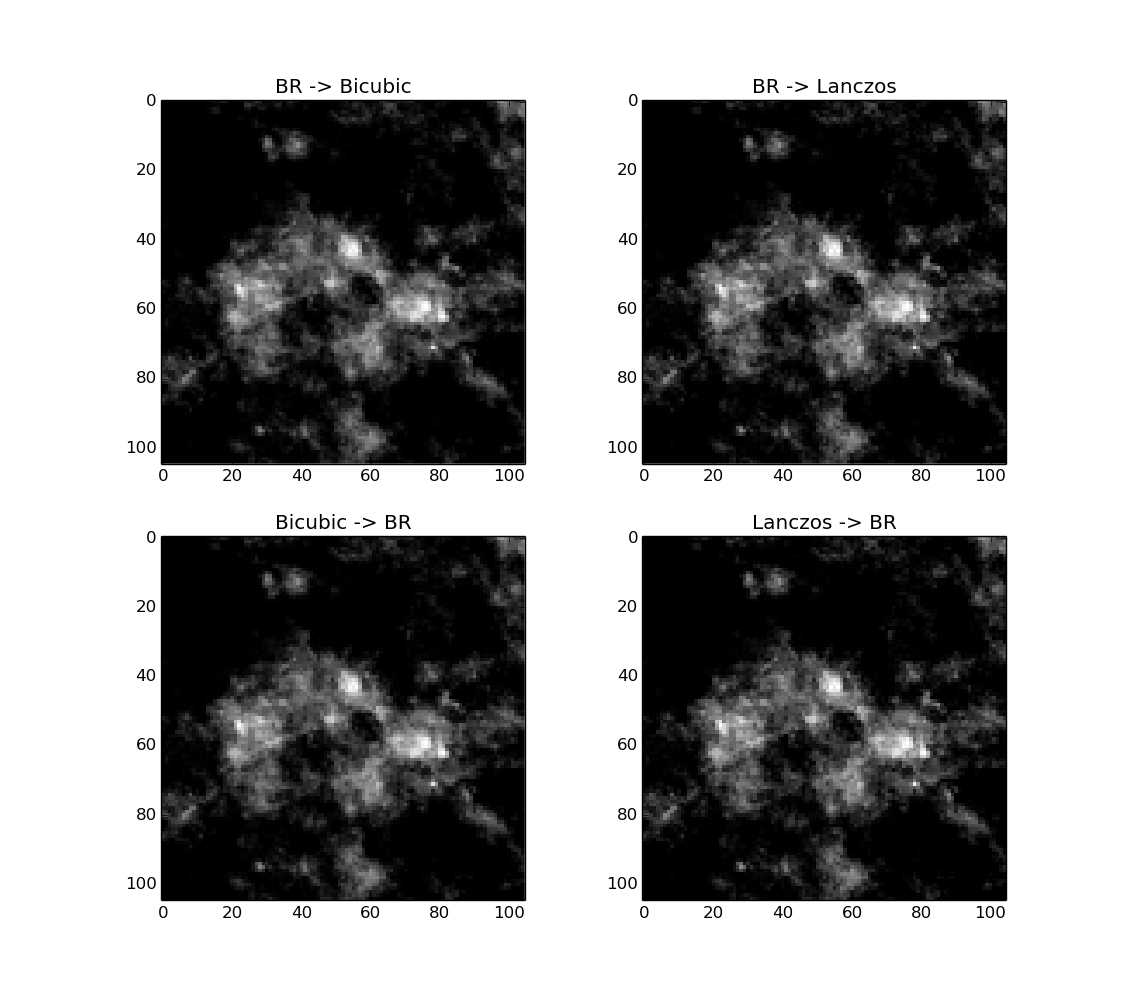
\includegraphics [width = 0.8\textwidth]{plots/mcDiffResizings.png}
	\caption[Example of resizing schemes]{Example of different resizing schemes applied to an image with a cluster of microcalcifications. Bicubic and Lanczos inteprolation is used for resizing an original 317 pixel image to 105 pixels before and after enhancement (background reduction plus normalization) as shown by the arrows in the subtitles. Results are virtually undistinguishable.}
	\label{fig:ResizingInterps}
\end{figure}

\subsection{Background}
We crop the images to the nearest non-zero pixel in x and y.


% When cropping to breast area and reducing make sure the reduced area is a multiple of 16, or downsample first and make sure the to-be-cropped area is multiple of 16. This way we can recover exactly the input image by downsampling exactly by 16x. 


Mammograms capture images of the breast against a black background which covers a good part of the mammogram. We delete any image patch which is 25\% or more black. No important information is lost in this process because the same part of the breast which appears in a deleted patch also appears on other image patches with less black background. A remaining question is how will the trained convolutional network react when presented with an all black input, for example, when slided across the background of a test mammogram. In practice, however, this is not relevant because it is clear that no lesion could occur outside the breast. 

An alternative is to preserve all images and let the network learn that black images are negative examples but this seems rather wasteful.

% Or could I crop the figure closely to the background and then calculate over all spaces (nop). How do you backpropagate through this mask? Just assign perfect scores to evry position in your predictions that is background (check where is the background in the mask), that way it will be counted by normal gradient, but it will not contribute. I could add a layer at the end (or before the loss function), that sets the gradient to zero in the backwards pass if the position it is viewing is  a background pixel. that'll do it.
% Or i could assume that anythong under the global mean won't be a mass and then during classification and during training just set them to black/treat them as background (this owuld be the equivalent ot train them and test them only on those pixels that are greater than the global means0). But maybe this then reduces the data se too much and I won't learn. More or less half the values are gonna go to zero. I would need to create a label where evrything below the global mena is background (0), any lession is (1) and any other breats tissue  is (0.5). Overcomplicated, better let the network also see some black patches maybe that help it. do get rid of backgorund, though.

\subsection{Labels}
% Labels are background, lession and breast tissue.
Once each image patch is obtained we need to assign labels to it. All image patches are initially labelled as negative (or no lesion) and only those where a lesion is present are labelled as positive. There are many ways to define the presence of a lesion in an image: (1) if a percentage of the lesion, say 70\% or more, appears in the image, (2) if a percentage of the image is covered by the lesion and (3) if a part of the lesion appears in the middle of the image.

We have chosen the last option to define the presence of a lesion because of three reasons: it is simple to implement, it somehow includes the other methods given that when a lesion appears on the middle of the image patch the rest of it will probably also appear on that patch and finally it encourages the convolutional network to output true only when the lesion appears in the center of the patch but not anywhere else which may give us more granular results when using it on the entire mammogram. The downside is that when a lesion is found on the outside of the image patch (in a corner, for example) it will be labelled as a negative example in the training set and may difficult the learning because even though the lesion is there we are training the network to answer negatively; if this effect actually occurs is not clear. \cite{Ciresan2013} uses this method to label its image patches.

Using the first or second option is a viable alternative although they come with their own caveats, for instance, it could be hard to calculate the area of irregular objects or the lesion could be so big that even covering the the entire image patch area it would still not account for 70\%.

We will use the type of lession (mass, clustered microcalcifications or normal) and the malignancy (bening, malignant or nothing) to train our networks.
% For the detection case, we do not consider malignancy it is lesion vs normal, for diagnosis we only consider the malignant ones.
% LeCun says convnets like to have many categories because they can identify better features early in the processing. Maybe it is better to have the same convnet for different lessions.

Databases normally offer adittional information such as age of the patient, breast density, family clinical history, assesment of the subtlety and malignancy of the lesion, etc. This information could be used as complementary features before classification or as labels for the network. In this stage we use only the mammograms with the labels stated above (binary classification).

% when downsampling the labels make sure every pixel in the smaller image is a valid label, downsample to the same size of the mammograms, (predicted segmentations which are way smaller are going to be upsampled 16x or 8x depending on the network that generated them)


\subsection{Image enhancement}
In theory we want to perform classification on the raw images (without any preprocessing) so we store the raw image patches and their labels as the base training set and perform any image enhancements during training whenever possible. There is a set of simple contrast adjustments that could be applied: normalization assigns 0 to the minimum gray value in the image and 255 (or the maximum available value) to the maximum gray value in the image and stretches the rest of the values linearly, background reduction plus normalization is similar except that all values below a given threshold (the mean of all pixel values in the image) are mapped to zero and the rest is normalized effectively reducing all small variations in the background to black and histogram equalization which tries to distribute the gray values evenly on the histogram of the image. An example of each method is shown in Fig.~\ref{fig:PreprocessingTechniques}.
\begin{figure}[h!]
	\centering
	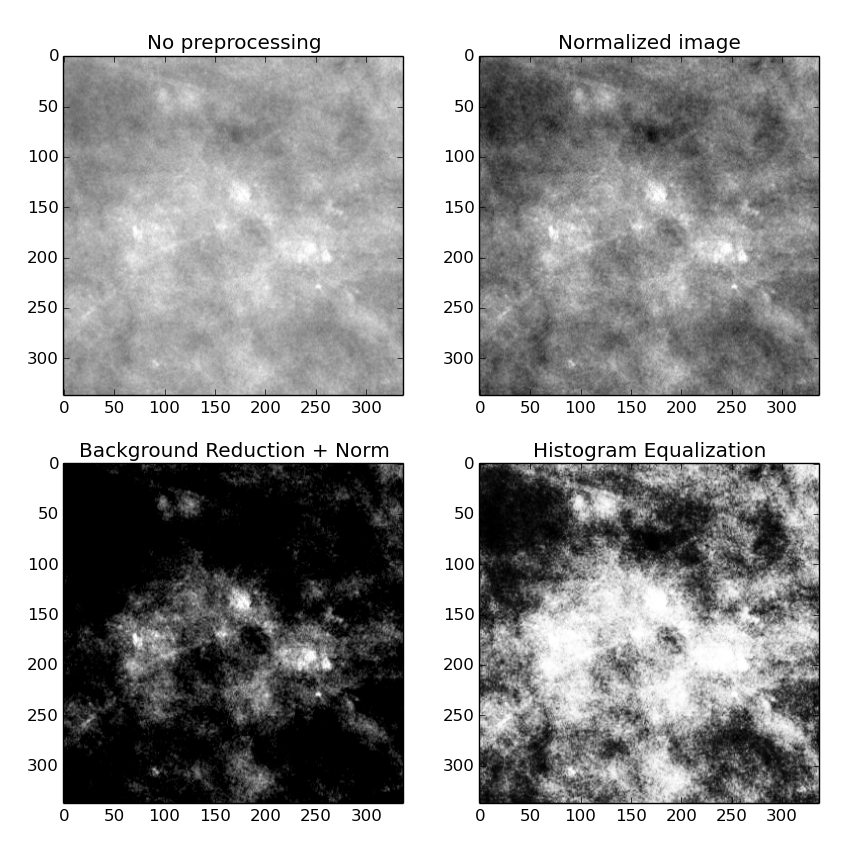
\includegraphics [width = 0.7\textwidth]{plots/mcDiffPreprocessings.png}
	\caption[Example of constrast adjustment techniques]{Example of simple contrast adjustment techniques applied to an image with a cluster of microcalcifications. Normalization takes the range of gray values and stretchs it up to linearly cover the entire range available. Background reduction assigns 0 to every pixel below the mean of the pixel values and applies normalization. Histogram equalization distributes the gray values more evenly in the histogram of the picture.}
	\label{fig:PreprocessingTechniques}
\end{figure}

We use background reduction plus normalization because it increases the signal to noise ratio, i.e., highlights lesions over normal breast tissue. On the downside, it also highlights dense structures (which could increase false positives) and may destroy important texture information by blending it with the background; using normalization only could produce better results. Unpreprocessed images seem too noisy and histogram equalization is too destructive for our purposes.

% Global contrast normalization makes comparisons across patients not good, because if a pixel is very bright in one patient that is only important with respect to that patient and it may end up (by contrast stretching) having the same value that the pixel in another mammogram who wasn't as bright but was the brightest of the mammogram. i think this makes sense because masss are going ot be bright but only in relation to the patient, maybe one has very fatty tissue so all is white and others have very clear tissue.
% You need zero-center so the gradients are computed properly.
% substracting bythe global mean counts as normalization (per-channel mean substraction), maybe i can subtract global mean and linearly stretch to -1 and 1. (Then to show the image i multiply by 127 and sum 127). Will it be the same result if I do contrast enhancement and then mean-center by subtracting 127 (now the range is -127 to 127). Make the calculus with constants. i think this is part of training.

% Try leaky relu (with alpha = 0.1), thay always give (slightly) better results, they don't kill the gradient in R- and are not zero-centered either.

% Idea: Look for a function that looks like a line, like a non-linear line. Becaus ewe want it to not zaturate on either side and to be zero-centered. something like x+sin(x), or 5x+xsin(x) this will be quasilinear but with change. that's exactly what i had in mind, but i don't think it will work. maybe somehting that grows to infinity but slowly sigmoid-shaped but it grows to infinty. also, what about reinitializing some neurons at random and retraining them. 

%TODO: Is feature normalization needed? It does put everything on -1 to 1 range (instead of 0-256, 0-2048, etc.). if it doesn't affect the results better do it

% show a figure with the original mammogram and what it wil look like after all this, and its labels.
	
\subsection{Data augmentation}
Rotations and flipping of original big images. the breast and cannals, and nipple may be very different at 90 and 270, flipping an 180 seem fine. Or maybe not.
We augment each enhanced image by using 4 rotations (at 0°, 90°, 180° and 270°) of both the original image and a horizontally flipped version of it, thus we increase our data set by a factor of 8. Both rotations and reflections preserve the original label. In principle it is not neccesary to store the augmented images because they can be easily generated during training but if the disk space is not prohibitive explicitly storing them simplifies training.
%Does it affect to present all different augmentations of the same image in one batch rather than in different batches?
% cutting mammograms in 4 or 16 pieces for training woul dnot be that bad, in fact as long as i overlap the regions a little bit and use no padding in the first layer (instead of padding it should have the original surrounding region, this is what decides what overlpas i need when i divide in 4 or 16). The results are gonna be exactkly as if i trained with every single patch in the image or with the entire image. This if i have no memory, or maybe if i wan to change up a bit. I would have to cut the labellings too, but that's not much o f aprobem as long as the training is the same as if it were end-to-end, which it is.

%\subsection{Storage} For each mammogram we will generate a 3-dimensional matrix ($x \times 64 \times 64$)  containing all $x$ preprocessed patches obtained from the mammogram and a 2-dimensional matrix ($x \times 4$) containing its respective labels. This matrices will be stored with the same name (plus a suffix) and on the same directory as the original image.


\section{Model}
We describe our chosen architecture and loss function.

\subsection{Architecture}
Following the recommendations from Section~\ref{sec:PracticalDL}, we define a simple network with six convolutional layers and two fully connected layers.

\begin{table}[h]
	\centering
	\begin{tabular}{lccccr}
	\hline
	\textbf{Layer} & \textbf{Filter} & \textbf{Stride} &\textbf{Pad} & \textbf{Volume} & \textbf{Params} \\
	\hline
	\texttt{INPUT}	& -	& - & - & $112 \times 112 \times 1$ & -\\
	\texttt{CONV -> LRELU} & $6 \times 6$ & 2 & 2 & $56 \times 56 \times 56$ & 2\,072\\
	\texttt{CONV -> LRELU} & $3 \times 3$ & 1 & 1 & $56 \times 56 \times 56$ & 28\,280\\
	\texttt{MAXPOOL} & $2 \times 2$ & 2 & 0 & $28 \times 28 \times 56$ & -\\
	\texttt{CONV -> LRELU} & $3 \times 3$ & 1 & 1 & $28 \times 28 \times 84$ & 42\,420\\
	\texttt{CONV -> LRELU} & $3 \times 3$ & 1 & 1 & $28 \times 28 \times 84$ & 63\,588\\
	\texttt{MAXPOOL} & $2 \times 2$ & 2 & 0 & $14 \times 14 \times 84$ & -\\
	\texttt{CONV -> LRELU} & $3 \times 3$ & 1 & 1 & $14 \times 14 \times 112$ & 84\,784\\
	\texttt{CONV -> LRELU} & $3 \times 3$ & 1 & 1 & $14 \times 14 \times 112$ & 113\,008\\
	\texttt{MAXPOOL} & $2 \times 2$ & 2 & 0 & $7 \times 7 \times 128$ & -\\
	\texttt{FC -> LRELU} & $7 \times 7$ & 1 & 3 & $1 \times 1 \times 448$ & 2\,459\,072\\
	\texttt{FC -> SIGMOID} & $1 \times 1$ & 1 & 0 & $1 \times 1 \times 1$ & 449 \\
	\hline
	\end{tabular}
	\label{tab:convNetArchitecture}
	\caption[Selected convolutional network architecture]{Architecture of the network used for experiments. It shows the filter, stride and padding used in each layer as well as the resulting volume and the number of learnable parameters per layer.}
\end{table}
% total # of parameters: 2 793 673

	The first convolutional layer uses a $5 \times 5$ filter with stride 2 (padding 2) to reduce the input spatial size from $127 \times 127$ to $64 \times 64$. After that all filters are $3 \times 3$ with stride 1 (padding 1), which preserves the spatial size and the pooling is $2\times 2$ stride 2 (padding 0) which reduces the spatial size by a half. This architecture has 4.63 million learnable parameters. 

	In case the input was size $64 \times 64$ pixels we could replace use a $3 \times 3$ filter with stride 1 in the first convolutional layer and leave everything else unchanged. For an all convolutional architecture we could replace all pooling layers by a $5 \times 5$ filter  with stride 2 and use input images of size of $113 \times 113$ or $129 \times 129$.

%	Leaky RELU

%subsection{Linear upsampling}
% For interpolations, see http://paulbourke.net/miscellaneous/interpolation/ y las definiciones de bilinear y bicubic above

\subsection{Loss function}
We downsample the labels rather than adding an upsampling layer. The loss function sums over all pixels in the breast area
% How do you backpropagate through this mask? Just assign perfect scores to evry position in your predictions that is background (check where is the background in the mask), that way it will be counted by normal gradient, but it will not contribute. I could add a layer at the end (or before the loss function), that sets the gradient to zero in the backwards pass if the position it is viewing is  a background pixel. that'll do it. If yu do judt kill the gradients of thebackground errors, try to report the loss function withouth those values, too, otherwise it will always overestimate the error. 
% If i Just multiply by the mask i can weight losses diferently.
% Make sure you count over everything that is  not backgorund and not just over everythingthat is 127, otherwise you may not count the lesion


\section{Hyperparameter selection}
We started with 30 networks ranged from 10 unif (-6, 0) for alpha and 10 uniform*-3,3) for lambda. Then refine this tranges to ...

\section{Training}
We offer details about the learning stage of our experiments.
% including hardware, software and optimization algorithms and other implementation notes.

\subsection{Hardware}
%Training neural networks is computationally intensive and requires equipment with powerful GPUs. 
We performed our experiments in 30 machines with the following specifications:
\begin{table}[h]
	\centering
	\begin{tabular}{cp{3.8cm}p{1.8cm}cc}
	\hline
	\textbf{Location}	& \textbf{GPU}	& \textbf{CPU} &\textbf{HD}	& \textbf{RAM}\\
	\hline
	%Personal	& Nvidia NVS 5400M \newline 96 cores, 1GB, compute capability 2.1 & i5-3210M \newline 2.5GHz & 57 GB & 4 GB\\
	A4-401 & Nvidia Quadro K620 \newline 384 cores, 2GB, compute capability 5.0 & i5-4570 \newline 3.2GHz	& 240 GB & 8 GB\\
	\hline
	\end{tabular}
	\caption{Available hardware for experiments}
\end{table}

Each computer was used independently to train networks (not distributed). Although we designed our models to be small enough to fit in the GPU memory, big images surpassed this storage limit causing errors; thus, we decided to train our networks only with the CPU. Training times ranged from 1 to 1.5 hours per 1000 examples.

\subsection{Software}
Models were implemented and trained using TensorFlow (v.11)~\cite{Abadi2015}. Tools for image retrieval, augmentation, evaluation and similar tasks were implemented in Python3.
Code, as well as trained models, are freely accesible at: \url{github.com/ecobost/cnn4brca}.

\subsection{Initialization}
Weights for the incoming connections to a unit are drawn from a normal distribution with zero mean and $\sqrt{2/n_{in}}$ standard deviation where $n_{in}$ is the number of connections. Biases are initialized to zero.

\subsection{Hyperparameter search}
\label{subsec:Hyperparameters}
We fit the learning rate and regulatization parameter simultaneously using random sampling. For each fold independently, we train 20 networks for five epochs (6\,520 examples) and select the best ($\alpha$, $\lambda$) combination using 20\% of the fold as a validation set. We use sensitivity at one false positive per image as performance metric.

\subsection{Optimization}
We use ADAM ($\beta_1 = 0.9$, $\beta_2 = 0.995$ and $\epsilon = 10^{-6}$) for optimization.
%, i.e., we perform stochastic gradient descent (with momentum and per-parameter adaptive learning rate).
Each parameter update uses the information from only a single training example but given that the loss is a weighted average over all pixels in the image, gradients are as rich as if we were performing mini-batch gradient descent with a batch composed of all image patches for which the network produced a prediction.

We trained the final model for all experiments for 30 epochs (49\,200 examples). No early stopping was performed.
% Any early stopping thing here


\section{Evaluation}
% Make sure the image inputted is grayscale, if not transform it, that way i can deal with color images, too.

\subsection{Post-processing}
Say that the logits out of the network were transformed intoprobabilities via softmax
Probabilities vs UNcorrected threshold vs Threshold and cluster extent correction vs threshold-free cluster enhancement vs, show different results at different thresholds
data is smooth, 

uncorrected threshold
Present the probabilities of tumor on each pixel. anmd threshold it on a given prob nd delete any clusters less than x.
Threshold free cluster enhancement (see module 29 in introduction to fmri)
Choose a threshold and delete any clusters less than x...

we could also present a heatmap with the different probabilities in each pixel of the image, for instance on mammograms we could present a grayscale image of whether a lesion is present.

% CRFs: public available implementation of (Krahenbuhl & Koltun)
% For the figure draw a random one  of 100x100 with a little signal in there and apply all corrections.

% Python implementation of CRF: https://pystruct.github.io/auto_examples/image_segmentation.html

% If using the threshold/ value under the cluster one, use the validation set t select pairs(threshold, total acceptable value)

% Background is thresholded at zero and shown in black

% Background is not counted to calculate the metrics. We use a mask to sum values only over the spaces that were a breast mass previously.

	\subsection{Evaluation}
	When dividing the data set we make sure \textit{all} image patches obtained from the same patient are assigned to either the training set or test set (not distributed) to avoid any possible overfit to the test set. Given that our data is unbalanced, with far more negative than positive examples, we use PRAUC (see Section~\ref{subsec:Classification}) to choose between models for hyperparameter selection and as an overall performance metric. Other metrics are also reported for completeness. 

	We could also evaluate the network on all augmentations of an image and output the average prediction; in theory, this would give us better results. For simplicity, we do not apply it for model selection.

	For detection of lesions on entire mammograms we slide the trained convolutional network across the mammogram computing a per-pixel prediction. The generated heatmap preserves the size of the original mammogram (with some zero-padding) and can be presented side to side to the original mammogram as a CAD system. In case this heatmap is noisy (predictions changes abruptly from pixel to pixel) we could use a median or gaussian filter to smooth it out.% We do not evaluate the network on the entire mammogram (or per patient), we limit ourselves to show the results.
	\subsection{Evaluation metrics}
F1-score AUc and those things are calculated only over breast tissue and lessions.
